\chapter{Introduction}
\section{Motivation}
The world wide web is a phenomenon of ever increasing dimension and integration into people's lives. In the beginning of 2019 roughly 4.3 Billion people had access to the internet which accounts for 56\% of the entire world population\footnote{https://www.internetworldstats.com/stats.htm\#links, accessed: 30.03.2019}. 
With more people being interconnected the amount of available data simultaneously increases. \\
This data consists of a broad spectrum of information people publicly or unintentionally share on the internet or more specifically among others through web-searches, blogs, chats, video games, online shops and social media platforms (SMP). SMPs provide services which allow users to create an online identity to present themselves to others by sharing personalised information. There are various SMP-providers available such as Facebook, Instagram or Twitter to name a few - all with their specific target audience and descriptive upload content. This social media data (SMD) is referred to as User Generated Content (UGC) or if it is georeferenced as Volunteered Geographic Information (VGI). VGI encompasses people's interests, performed activities, future intentions, sense-of-place and perception of locations \parencite{Goodchild2007}. This geotagged information as it is also known allows for spatial mapping of data in space.  
According to the Federal Statistical Office (FSO) of Switzerland 73\% of people between the age of 16 and 74 were in the year 2017 in the possession of a smart mobile device\footnote{https://www.bfs.admin.ch/bfs/de/home/statistiken/kultur-medien-informationsgesellschaft-sport/informationsgesellschaft/gesamtindikatoren/haushalte-bevoelkerung/mobile-internetnutzung.html, accessed: 30.03.2019}. These devices are generally equipped with the Global Positioning System (GPS) which supports the provision of VGI.
This social media derived big-data holds a lot of potential for various research applications as already highlighted by papers such as \textcite{DiMinin2015, DiMinin2017, Meentemeyer2016}. The main advantages to conventional methods such as surveys and interviews are comparably fast, (mostly) easy and low-priced continuous data-streams as well as a good spatial and temporal coverage at multiple scales.\\
\newline
Also a phenomenon of modern times are increased rates of job induced mental fatigue, stress and illness which are side products of an ever more specialised and demanding economy. To address that issue the report of mental health in Switzerland \parencite{Ruesch2003} was conducted among others by the Federal Office for Public Health (FOPH) which highlights the lack of prevention measures in place. This led to a monitoring program to foster mental health provision and awareness in Switzerland \parencite{Schuler2012} also on a cantonal level. The environment is known to be a sustainable source for mental health benefits by providing a diverse range of recreation possibilities. The extent and potential value associated with these provided ecosystem-services was noted in the 'effects of the environment on human health' report \parencite{Ragettli2017} of the Federal Office for the Environment (FOEN). \\

\section{Problem statement and aim}
Identifying and mapping activities related to nature-based recreation, outdoor recreation or soft ecotourism as described by \textcite{Deng2002, Balmford2009} is the aim of this thesis.
Increasing the quality, quantity and attractiveness of nature-based recreation requires knowledge over the current usage of space. More specifically, in regards to the activities people perform in the environment to answer the following questions: (1) What nature-based recreation activity (NBRA) should be promoted in a certain area and (2) what kind of supportive infrastructure should be constructed to maximise its utilisation? This thesis tries to respond to that current need for information by investigating the potential of SMD in particular from the SMPs Instagram\footnote{https://www.instagram.com/} and Flickr\footnote{https://www.flickr.com/} for analysing and monitoring the spatial occurrences of NBRAs including walking, hiking, jogging, biking, dog walking, horse riding and picnicking in the Canton of Zug, Switzerland. The mentioned SMPs are known for hosting geotagged images with attached user-generated text (for more detailed information refer to section \ref{data_acquisition}) and were proven to be good indicators for multiple applications such as determining visitation rates to nature reserves \parencite{Tenkanen2017, Heikinheimo2017, Keeler2015, Wood2013} or to social events \parencite{Pettersson2011}, human mobility patterns \parencite{Barchiesi2015, Grossenbacher2014} and recreation locations \parencite{Weyland2014, Hill2006, Neuvonen2010}.
Accordingly, this study tries to evaluate the potential of SMD as a proxy for predicting the occurrences of NBRAs as an alternative to conventional data-acquisition methods such as surveys is investigated.\\
The goal of achieving a comparison between the people's usage of space and the already present infrastructure to evaluate an efficient asset allocation was performed with the data of the web-application Foursquare\footnote{https://de.foursquare.com/}. This data consists of categorised infrastructural elements also known as \textit{venues} which were used as indicator for the current dispersion of sport and recreation facilities in the research area. The results of this comparison aim to improve spatial planing by optimising the allocation of recreational infrastructure in correspondence to the where people actually perform certain NBRAs.

\section{Approach}
The approach presented in this thesis creates and evaluates two machine learning (ML) models to predict NBRAs in georeferenced Instagram and Flickr posts. These posts are referred to as media objects throughout the thesis. The first model is trained on a combination of text and image data which has not in this way been done before. The second model was solely trained on text data and functions as a baseline reference to investigate the effect of including image content information. Structural image elements are extracted with the help of a deep-learning algorithm named Google Cloud Vision as also used by \textcite{Richards2018}. The models are individually trained on 1'046 manually classified Instagram media objects originating from a dataset of the region of Zurich \parencite{Gruzd2016} and tuned for best performance. Classification specific model evaluations are subsequently manually conducted on the NBRA-predictions in the research area located in the canton of Zug to compare the two finalised model performances based on untrained data. The innovation of this approach lies in the fully automated prediction process without any manual content analysis which uses dominantly openly accessible and free software. This shall pave the way for a feasible reconstruction and application by e.g. municipal authorities or agencies with a low budget for high priced software licences. \\
\newline
In the course of this thesis, additional ground truth data from interviews and passive observations was acquired in three locations of the research area. The interviews were used to gain insight on three topics. Firstly the drivers that motivate people to visit certain locations above others. Secondly the social media usage of the interviewees in terms of SMP-engagement, upload-frequency and behaviour. Lastly some personal details were recorded which were kept anonymous to gain information about the demographics of social media users. The passive observation as second part of the ground truth was used to count NBRAs-occurrences during the time the interviews were held. In the end the ground truth derived signals were compared to the SMD to evaluate and justify the ML models legitimacy.


\section{Background of machine learning}
This section is laid out to give the reader a short introduction into the field of machine learning (ML) as well as a basic understanding of associated terminologies to help comprehend the applied approach of this thesis.\\
ML in its core refers to the process of a computer to understand or 'learn' the relationships inside a dataset with the help of algorithms to be able to make predictions on data the model has never seen before.
The training's data normally consists of different features which identify and characterise a given entry. The constellation of feature-values which can be metaphorical seen as a 'fingerprint' of a given data point are the reason why a model can potentially make out patterns and relate them to a certain output. This output can either be a class (in the case of a classification problem) or a continuous number (in the case of a regression problem) of new data point.
An example of potential features of a regression problem could be different body measurements of a specific animal with the aim to differentiate between different types of the same species. The training's data would then consist of multiple entries where most likely a human measured the needed body parts of several individuals and entered the continuous numerical value in the corresponding feature field.\\
\newline
One can differentiate between two types of ML - supervised and unsupervised learning. To illustrate the difference imagine a set of training's data where each entry is represented by a point in an n-dimensional space where \textit{n} corresponds to the number of features present and the coordinates of each point (position vector of that point) correspond to the feature's values. If we make the link back to the example above then unsupervised learning would mean that the training's data consists of only the training's data without any labels. The labels in this case would have been the names of the animal species that the measurements were taken from. In this way the model is forced to find natural breaks / boundaries on its own in the training's data by clustering similar data points together and regarding them as an independent class. The hypothesis here is that points closer to each other in space are more related to one another than distant ones - similar to the first law of geography. These model given class names do not correspond in any way to the actual names of the animals because the model has no information on it what so ever. It is up to the user to appropriately label the clusters / classes the model isolated.

\begin{figure}[h]
   \centering
   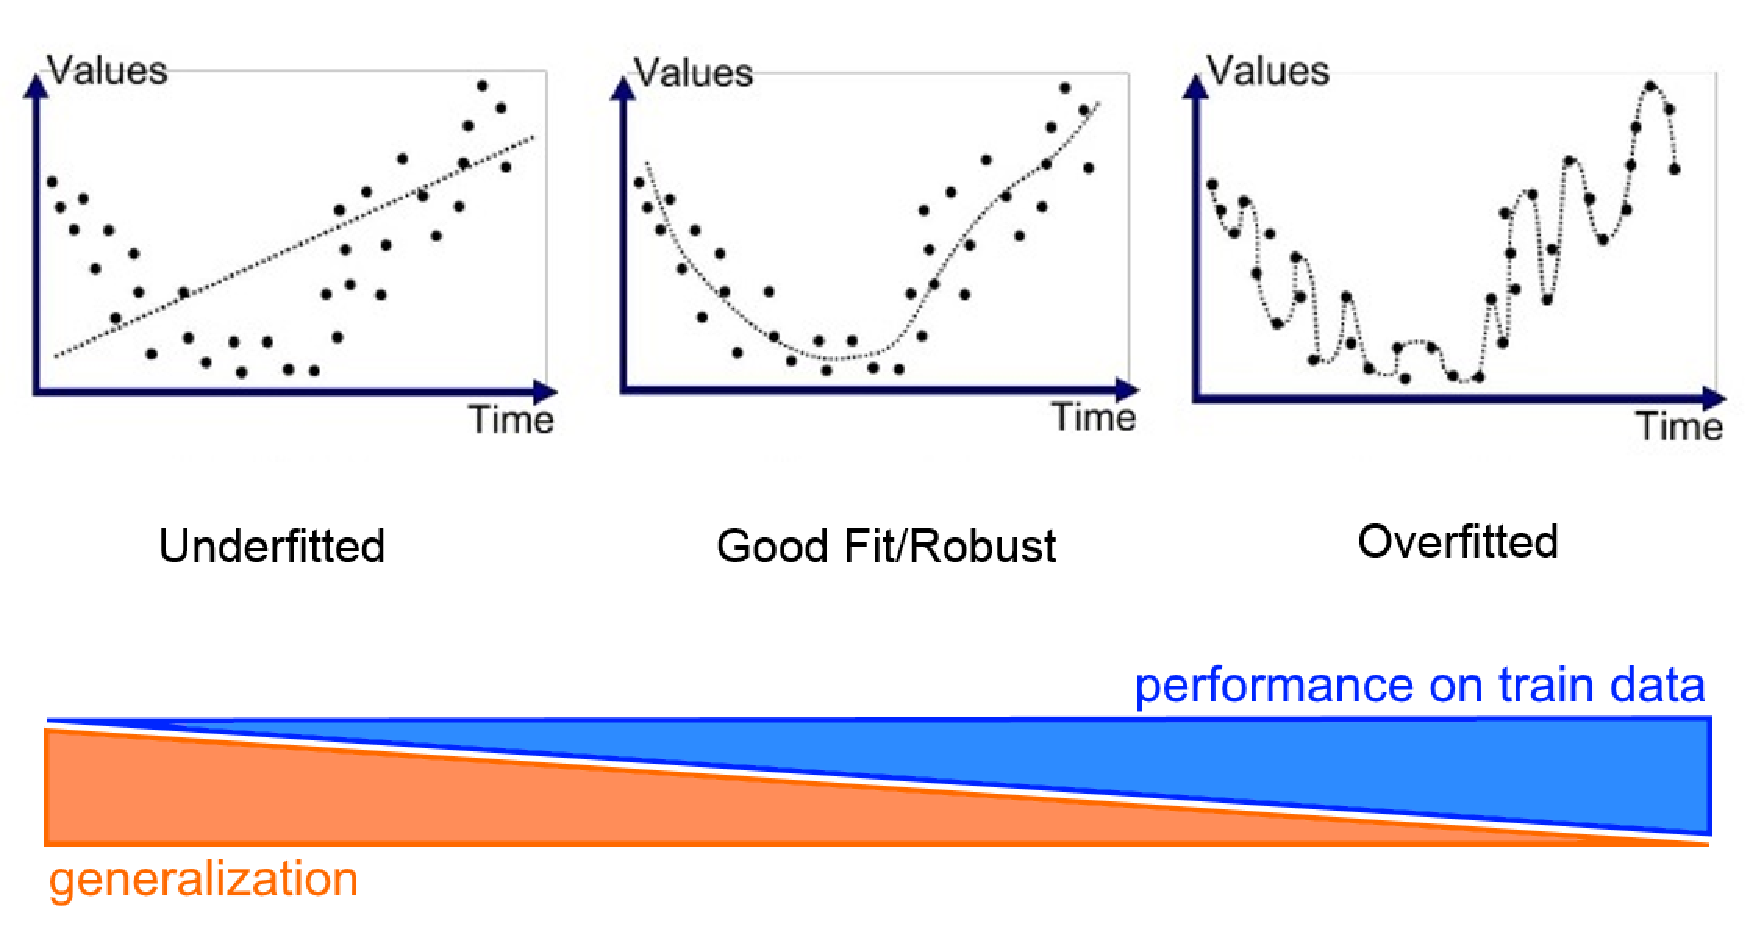
\includegraphics[width=\textwidth]{img/over_underfitting}
   \caption{Visualisation of under- and overfitting on a dataset.}
   \source{altered by the author, https://medium.com/greyatom/what-is-underfitting-and-overfitting-in-machine-learning-and-how-to-deal-with-it-6803a989c76, accessed: 29.03.2019}
   \label{fig:over_underfitting}
\end{figure}

Supervised learning on the other hand happens when the model is fed and trained upon example data with their correct classification labels present. The term 'supervised' therefore relates to the fact that presumably a human told the model which data points belong to which class. This approach is understandably more laborious because the creation of a labelled training's dataset takes time. The benefits are generally better performing models and the possibility to directly test the model. The testing is done by splitting the original training's dataset into two parts. Generally, a bigger portion ($\sim$ 75\%) is used for training the model and the other one ($\sim$ 25\%) - which the model has never seen during the fitting phase - is used to test the model's performance. \\
\newline
Frequently used terms in relation to ML are under- and overfitting. These terms correspond to two extremes of how the model and its incorporated (boundary-) function is fitted to the provided test-data (see points in figure \ref{fig:over_underfitting}). Underfitting describes the state, where the model does not seem to extract and comprehend any logic from the dataset and therefore over-generalises the classification or regression problem at hand (see outer left graph of figure \ref{fig:over_underfitting}). \\
The other extreme is known by the term overfitting where the model tries to correctly classify every single training-data point to its proper class. This results in the model being extremely tuned to the provided training-data but not being able to generalise well on new unseen data (see outer right graph in figure \ref{fig:over_underfitting}). In other words overfitting basically means that the model learned the training's data by hard which results in misleadingly high performance scores. The process of finding the balance between a model that is able to generalise on new data while identifying the underlying data-patterns is further described in section \ref{ml_text_data}.

\section{Ethics}

Drawing upon crowed sourced big-data is inevitably shadowed by ethical controversies. Using GPS locations and other sensitive data to identify and analyse patterns of human behaviour is rightfully criticised and sometimes considered unethical practise.\\
We are only talking about data that is publicly available, data that the user decided to share on the web on his or her own behalf - or is it?. The paper of \parencite{Estima2016} shows that not the entirety of data is voluntarily shared. Did the user sign up for his or her data to be systematically analysed? This depends on the Terms of Service (TOS) of the corresponding SMP which are hardly ever read by the consumer.\\
One has to understand the potential power this data possess. Having access to hundreds of personalised media objects of a specific social media user enables analytics to construct a blueprint of that person. This blueprint can encompasses the persons political orientation, its home and work location, preferences and dislikes as well as daily routines. Personalised advertisement would then be the smallest resulting threat. Interpersonal surveillance \parencite{Trottier2017}, stalking \parencite{Lyndon2011} or potential blackmailing through acquired sensitive information are by far greater and current threats. Additionally, it is unclear from a data-researcher point of view how to deal with encounters of media objects that indicate illegal behaviour e.g littering, assault or theft.\\

With that being said I personally think that the ethical discrepancy is legitimately continuously discussed in this context. Showing how the data and the anonymity of the authors is treated as well as the goal a project pursues are key elements that determine in my opinion if ethical terms are violated or not. 






